\documentclass[minf,frontabs,twoside,singlespacing,parskip]{infthesis}

\usepackage[xetex]{graphicx}
\usepackage{fontspec,xunicode}
\defaultfontfeatures{Mapping=tex-text,Scale=MatchLowercase}
\setmainfont[Scale=.95]{Georgia}
\setmonofont{Georgia}

\usepackage{amsmath}
\newcommand{\BigO}[1]{\ensuremath{\operatorname{O}\bigl(#1\bigr)}}

\begin{document}

\title{Modelling search volumes as a dynamic system responding to external events}

\author{Stefan Sabev}

\course{Master of Informatics}
\project{{\bf MInf Project (Part 1) Report}}

\date{\today}

\abstract{
It is well known that some events might spark people's interest to fly to different destinations. In particular news events or sports events can quite easily make people search for a specific destination - for example the Champions League Quarter final draw increased the number of flight searches from Glasgow to Spain 6 times.
The main goal of this project is to collect Twitter data initially and possibly several other news sources and extract the available event data. Afterwards we'd want to split it into two groups - those who spark people's interest and those don't.
This can later be used to detect when people want to go somewhere based on the news channels around the world.
}

\maketitle

\section*{Acknowledgements}
Acknowledgements go here. 

\tableofcontents

\pagenumbering{arabic}

\chapter{Introduction}

In recent times social media has been of great interest to everyone. Everyone is trying to benefit from the vastness of the data available - companies are paying for sentiment analysis, targeted ads, promoted trends and so on. 

With a base of 190 million active monthly users, Twitter{\copyright} has turned into quite an promising source of data. Many are trying harness the power of social media and use it to some purpose - to see how their product or company is performing or predict something about the future such as flu outbreaks, etc.

The aim of this dissertation is to explore the effect that social media, and more specifically Twitter, has over online travel. The aim is to show that using Twitter we can build a model that will be able to predict certain shifts in demand on some airline routes. In order to do this, we will employ a basic event detection mechanism, which will alert every time something odd happens for a particular destination and subsequently try to match that to a change of flight search profile. 

\chapter{Data collection}

The first and most important part of this project was to start collecting the correct data, which was to be used in building the model later. Twitter offers quite a comprehensive API with a lot of attributes, however in order to reduce the daily volume of data I had to take the most relevant ones for me. 

The attributes chosen to collect are:
\begin{itemize}
\item Text - the text of the tweet is the most important one, perhaps. Quite a lot of information can be extracted from it alone
\item Id - the tweet id. Useful if we want to screen scrape for any additional information or just to provide a tidy small dataset of ids.
\item ID Str - String representation of the above.
\item Source - What is used to post the tweet. The Twitter website is marked as "web".
\item Coordinates  - Representation of the geographical location of the Tweet as reported by the utility used to post the tweet.
\item Entities - This include hashtags, user mentions and urls included in the tweet. Could be taken from the text, but it's nicer to have them ready.
\item Retweet count - the number of times the tweet was retweeted. Useful for any future models. 
\item Favourited - Indicates whether the tweet was retweet by people. 
\item Language - The language of the tweet. We should be capturing English only, but put in place for future expansion into the multi-language domain
\item Filter level - indicates the level of filtering applied to the stream.
\item Place - Shows where the tweet was tweeted from. Gives more detail than coordinates - country, city name, coordinates as well. Not necessarily available for all tweets.
\end{itemize}

The first stage of the project is to look only at tweets in English from the UK. The second stage would be to develop the model even further and add multi-language and multi-country support. 

By selecting those particular tweet attributes and using the Streaming API, I managed to reduce the daily volume of data from \textasciitilde 6GB of data down to \textasciitilde 3.5GB/day.
The amount of data accumulated at the time of writing is \textasciitilde 360 GB. The collector has been running successfully from September 2013, however there are some holes of the data caused by network outages or the script interacting with the Twitter Streaming API crashing. 

The data on flight search volumes is kindly provided by Skyscanner. In order to ensure that there are no concerns with confidentiality I have anonymised the data. 



\chapter{Exploration and analysis of the data set}

Since we have a completely new problem at hand here there is a lot of exploration of the data sets required to understand what we can do with them.

I have tried several different approaches to filtering the data and exploring the relationship between the multiple variables. A brief summary of those would be:
\begin{itemize}
\item Using hashtags which contain a country or city name and taking their counts.
\item Taking every tweet that has a city/country name in its text in a conduction with a travel related term from the list. 
\end{itemize}

Another important aspect of the project is to take care of the data. Because of some teething problems both with the Skyscanner data and the Twitter Streaming API, there are some holes in it, which I have chosen to remote by filling in data generated by the Last 4 Fridays forecasting method. 



\section{Hashtags}

Hashtag is one of the most important constructs by Twitter. Here's an example tweet:

\begin{quotation}
@FunnyChap: Something witty and very well said \bf{\#jokeoftheweek}
\end{quotation}

The user who has tweeted is denoted with a @ before the username. A hashtag is usually a single word with a \# before it. 
You can filter out and explore twitter content based on hashtags and usually every major event has its own hashtag. The ones which are most mentioned appear in a special section called "Trending".

This option was considered, because if it had worked it would have been what we would call a "quick win". It doesn't require much processing, since what you'd need is just take the ready made list of hashtags and store all the results into a in-memory dictionary, which you'd then split by city/country. That reduced the overall size of the relevant tweets to \textasciitilde 3 GB. What was even greater is that we didn't really require the text information itself, which made the working dataset even smaller. 

However the overall counts yielded to be quite smaller and the distribution of the values was quite random, which means that fitting a model to this would've been quite tricky. 

\section{Occurrences paired with travel terms} 

The next slightly more expensive in computation terms option was to look at the actual tweet content and to count the number of times a city/country name appeared in conjunction with a one word form a list of travel-related words:

\begin{quotation}
terms = \\
\{ "airport": "", \\
"check-in": "", \\
"fly": "", \\
"land": "", \\ 
"landing": "", \\
"plane": "", \\ 
"take off": "", \\
"destination": "" \\
... \}
\end{quotation}

The list is modelled as a dictionary, because dictionary lookups are \BigO{1}, so iterating over the words in the tweet and checking whether they appear in the city/country dictionary or the travel terms proved to be the most efficient combination.

\section{Finding the correlation between those variables}

The easiest way to test the statistical correlation between your data would be to carry out the Pearson test.

For London the numbers we got back from that are:
\begin{quotation}
In [39]: r\_row, p\_value

Out [39]: (0.13, 0.28)
\end{quotation}

From this it seems that the situation is truly unrelated. After all a positive correlation of only 13\% is something that even a social scientist wouldn't report!

However, when you plot the two things we are trying to correlate something a bit more interesting comes up:

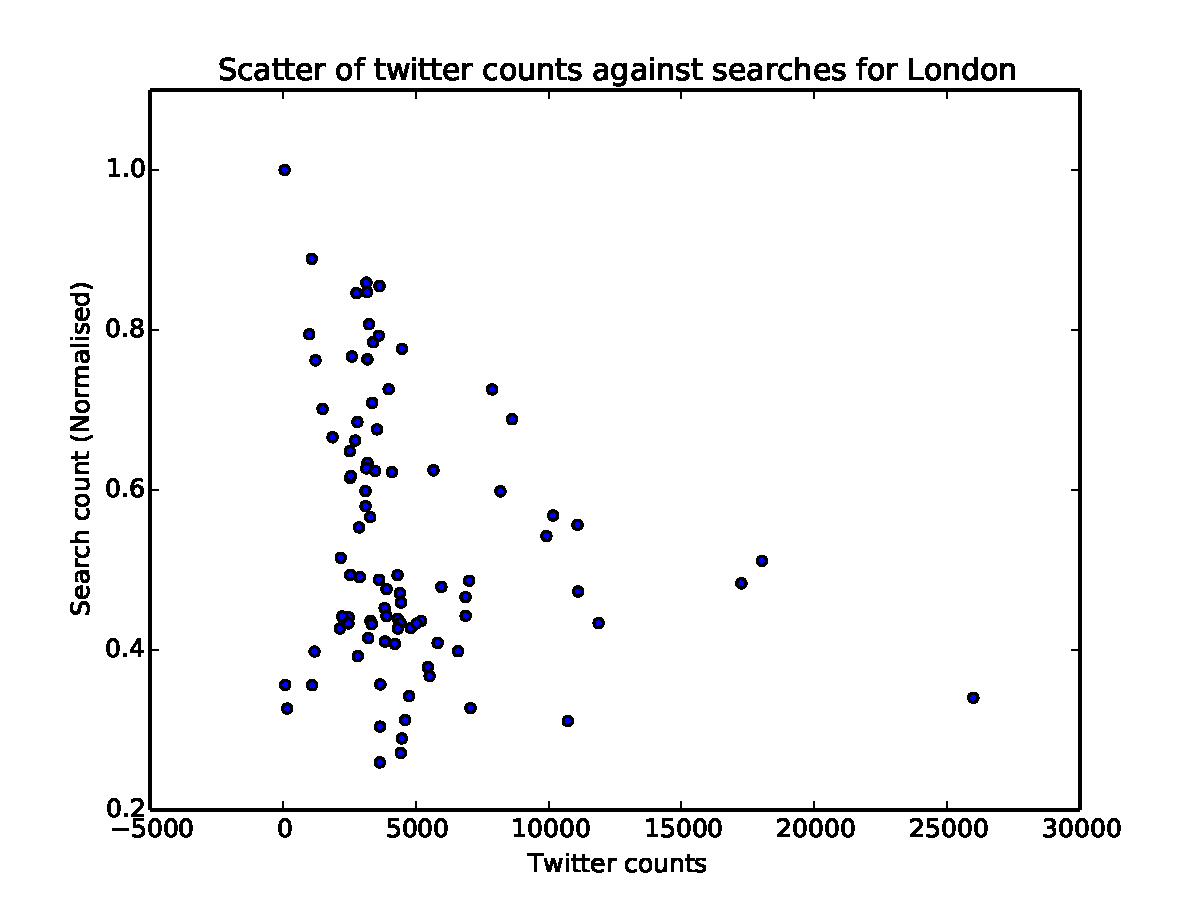
\includegraphics[width=\textwidth]{scatterv1}

There is definitely a relationship, even though not perfectly linear.

We can observe that there is a well defined cluster where the twitter counts are quite high, but the number of redirects is quite big. So we can certainly say that those variables are correlated, but the outliers push the coefficient down quite a significant amount. The interesting part of this scatter plot for us is the top right corner. We are interested in those abnormal Twitter counts, which correspond to high number of redirects. Another interesting thing to explore would be to see if we correlate the mentions on the social network with the redirects from the next day. That will assume a certain lag factor, which is reasonable as sometimes an event should not effect the redirect counts till the next day when it's picked by all the major media.

The next city, which would have been interesting to explore is Sydney, since the Pearson coefficient there is even smaller - only 4\% positive correlation. 

The Pearson test yields the following values for Sydney:
\begin{quotation}
In [23]: r\_row, p\_value

Out[23]: (0.05, 0.70)
\end{quotation}
\newpage
And here is the scatter plot:

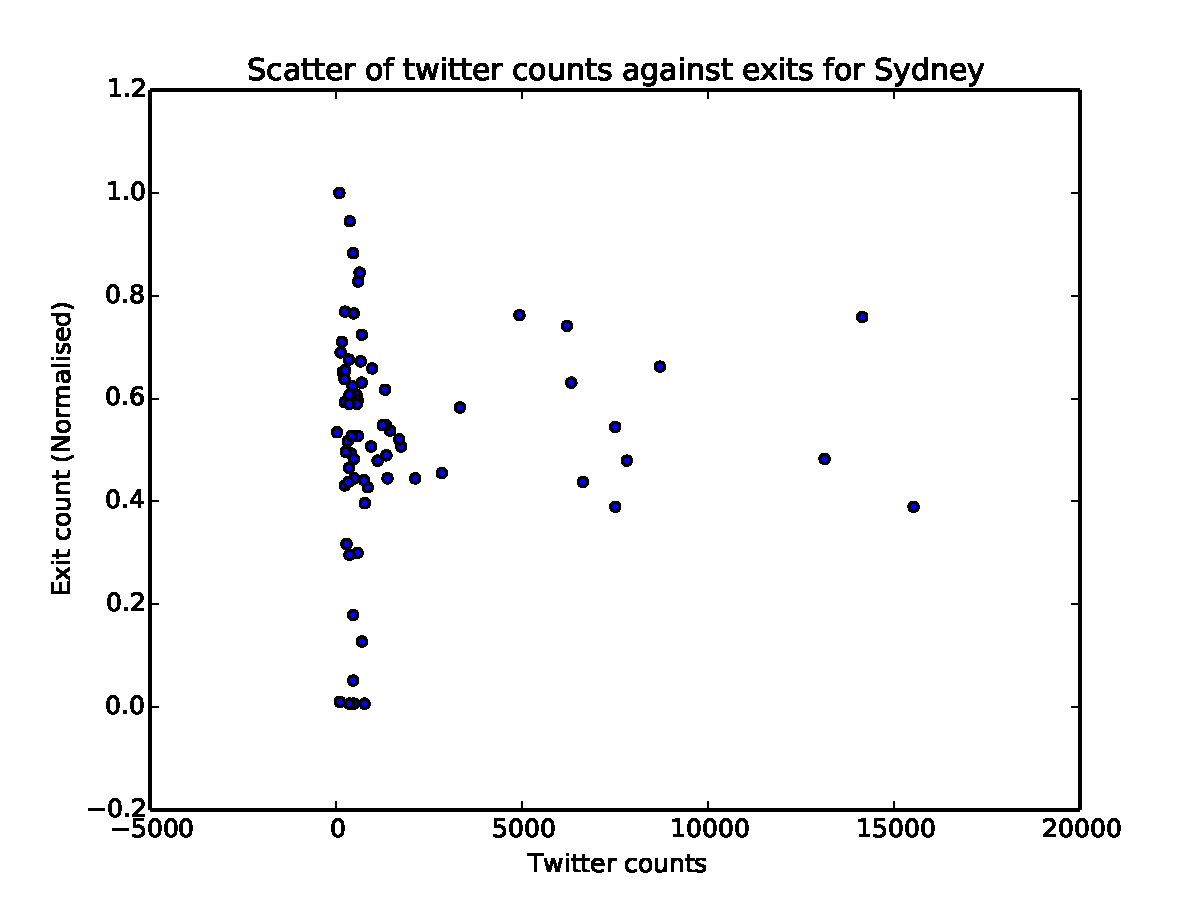
\includegraphics[width=\textwidth]{Sydney_scatter}

Here we do see that indeed the correlation is not as well expressed. The implications of that are that the approach we take to building the model must be more versatile - we will aim to build one model for the overall twitter counts of places correlated to the total number of exits and models on a per city basis.

\section{Cleansing the data}

As mentioned,every time you depend a few external data source there will be some holes in the data, caused by several things. 

In my case they were a couple of major sources of risk:
\begin{enumerate}
\item The script that collects data from the Streaming API.
\item The searches data coming from Skyscanner being incorrect or partial - not spanning the full date range.
\end{enumerate}

The dates with incomplete data or missing data altogether can seriously impact any regression or statistical test, so it was vital to tidy up the data set by backfilling the data. I applied the Last 4 Fridays mentioned in the following chapter in order to make the dataset more consistent and easier to work with. 

The interesting part was that it completely change the results from the test. For London the values returned by the Pearson test are now:

\begin{quotation}
In [23]: r\_row, p\_value

Out[23]: (-0.23, 0.02)
\end{quotation}

That is quite interesting and it has a lot of implications on the models we will use afterwards to correlate the two variables. 
We might have to add a certain "lag" factor to this, which will offset the tweets by correlating the numbers extrapolated from Twitter with the numbers and match them against searches from the following day.

\section{Top features} 

The idea here is to extract the top N features from the tweet and use them in the logistic regression model that we will build to predict the 



\chapter{Models}

\section{The baseline model}

The baseline model for predicting the number of redirects Skyscanner has on a daily basis is called Last 4 Fridays. 
It works in the following way:
\begin{enumerate}
\item We want to predict the number of redirects/searches for this Friday.
\item We take the number of redirects/searches Friday from last week, the week before, etc, until we have the counts form the previous 4 weeks for the corresponding day.
\item We then assign weights to those 4 numbers and assign weights - the most recent one will get the highest weight, the one after about a half and so on. The exponential weighting scheme captures short term seasonality.
\end{enumerate}

This model was tested out against more complex classifiers like ARIMA and Autoregressive Vector Methods and it performed really well, but unlike the others it was many times simpler to program and maintain.


\chapter{Timeline}

The timeline for the next 3 months is the following:
\begin{enumerate}
\item Continue with the tests
\item Chose which approach is to be picked up:
\begin{itemize}
\item Explain spikes in searches by looking at historical tweet data
\item Or try to predict the spikes in the first place
\end{itemize}
\item Final draft done by mid-March.
\item Submit dissertation.
\end{enumerate}


%\begin{thebibliography}{50}
%\bibitem{1} Twitter Stats \textsl{\href{http://www.statisticbrain.com/twitter-statistics/}{Twitter Stats}}
%\bibitem{2}  API Documentation \textsl{\href{https://dev.twitter.com/docs/streaming-apis}{Streaming API}}
%\end{thebibliography)

\end{document}
